%!TEX root = ../Thesis.tex
%% Basierend auf TeXnicCenter-Vorlage von Mark Müller
%%                      Willi Nüßer
%%                      Waldemar Penner     
%%                      Ulrich Reus
%%                      Frank Plass
%%                      Oliver Tribeß 
%%                      Daniel Hintze     
%%%%%%%%%%%%%%%%%%%%%%%%%%%%%%%%%%%%%%%%%%%%%%%%%%%%%%%%%%%%%%%%%%%%%%%

% Wählen Sie die Optionen aus, indem Sie % vor der Option entfernen  
% Dokumentation des KOMA-Script-Packets: scrguide

%%%%%%%%%%%%%%%%%%%%%%%%%%%%%%%%%%%%%%%%%%%%%%%%%%%%%%%%%%%%%%%%%%%%%%%
%% Optionen zum Layout des Artikels                                  %%
%%%%%%%%%%%%%%%%%%%%%%%%%%%%%%%%%%%%%%%%%%%%%%%%%%%%%%%%%%%%%%%%%%%%%%%
\documentclass[%
paper=A4,         % alle weiteren Papierformat einstellbar
fontsize=12pt,    % Schriftgröße (12pt, 11pt (Standard))
BCOR=12mm,         % Bindekorrektur, bspw. 1 cm
DIV=14,            % breiter Satzspiegel
parskip=half*,    % Absatzformatierung s. scrguide 3.1
headsepline,      % Trennline zum Seitenkopf  
%footsepline,     % Trennline zum Seitenfuß
%normalheadings,  % Überschriften etwas kleiner (smallheadings)
listof=totoc,     % Tabellen & Abbildungsverzeichnis ins Inhaltsverzeichnis      
%bibtotoc,        % Literaturverzeichnis im Inhalt 
%draft            % Überlangen Zeilen in Ausgabe gekennzeichnet
footinclude=false,% Fußzeile in die Satzspiegelberechnung einbeziehen 
headinclude=true, % Kopfzeile in die Satzspiegelberechnung einbeziehen 
final             % draft beschleunigt die Kompilierung
]
{scrartcl}

%\setuptoc{toc}{totoc} % Inhaltsverzeichnis ins Inhaltsverzeichnis

% American English
\usepackage[american]{babel}

% Umlaute können verwendet werden
\usepackage[utf8]{inputenc}   

% Echte Umlaute
\usepackage[T1]{fontenc} 

% Latin Modern Font, Type1-Schriftart für nicht-englische Texte
\usepackage{lmodern} 

% 1/2-zeiliger Zeilenabstand
\usepackage[onehalfspacing]{setspace}

% Für die Defenition eigener Kopf- und Fußzeilen
\usepackage{fancyhdr} 

% Für die Verwendung von Grafiken
\usepackage[pdftex]{graphicx}

% Bessere Tabellen
\usepackage{tabularx}

% Für die Befehle \toprule, \midrule und \bottomrule, z.B. in Tabellen 
\usepackage{booktabs}

% Erlaubt die Benutzung von Farben
\usepackage{color}

% Verbessertes URL-Handling mit \url{http://...}
\usepackage{url}

% Listen ohne Abstände \begin{compactlist}...\end{compactlist}
\usepackage{paralist} 

% Ausgabe der aktuellen Uhrzeit für die Draft-Versionen
\usepackage{datetime}

% English quotes
\usepackage{csquotes}

% Konfiguration der Abbildungs- und Tabellenbezeichnungen
\usepackage[format=hang, font={footnotesize, sf}, labelfont=bf, justification=raggedright,singlelinecheck=false]{caption}

% Verbessert die Lesbarkeit durch Mikrotypografie
\usepackage[activate={true,nocompatibility},final,tracking=true,kerning=true,spacing=true,factor=1100,stretch=10,shrink=10]{microtype}  

% Zitate und Quellenverzeichnis
\usepackage[
    bibstyle=authoryear,
    citestyle=ieee,  
    giveninits=false,         % false = Vornamen werden ausgeschrieben
    natbib=true,
    urldate=long,             % "besucht am" - Datum
    %url=false,
    date=long,                
    dashed=false, 
    maxcitenames=3,           % max. Anzahl Autorennamen in Zitaten
    maxbibnames=99,           % max. Anzahl Autorennamen im Quellenverzeichnis
    backend=biber
]{biblatex}
  
% Bibliograpthy
\bibliography{library/library}

% Keine Einrückung bei einem neuen Absatz 
\parindent 0pt 

% Ebenentiefe der Nummerierung
\setcounter{secnumdepth}{3}

% Gliederungstiefe im Inhaltsverzeichnis 
\setcounter{tocdepth}{3} 

% Tabellen- und Abbildungsverzeichnis mit Bezeichnung:
\usepackage[titles]{tocloft}

% Sourcecode-Listings
\usepackage{listings}

% Bestimmte Warnungen unterdrücken
% siehe http://tex.stackexchange.com/questions/51867/koma-warning-about-toc
\usepackage{scrhack} 

%% http://tex.stackexchange.com/questions/126839/how-to-add-a-colon-after-listing-label
\makeatletter
\begingroup\let\newcounter\@gobble\let\setcounter\@gobbletwo
  \globaldefs\@ne \let\c@loldepth\@ne
  \newlistof{listings}{lol}{\lstlistlistingname}
\endgroup
\let\l@lstlisting\l@listings
\makeatother

\renewcommand*\cftfigpresnum{Figure~}
\renewcommand*\cfttabpresnum{Table~}
\renewcommand*\cftlistingspresnum{Listing~}
\renewcommand{\cftfigaftersnum}{:}
\renewcommand{\cfttabaftersnum}{:}
\renewcommand{\cftlistingsaftersnum}{:}
\settowidth{\cftfignumwidth}{\cftfigpresnum 99~\cftfigaftersnum}
\settowidth{\cfttabnumwidth}{\cfttabpresnum 99~\cftfigaftersnum}
\settowidth{\cftlistingsnumwidth}{\cftlistingspresnum 99~\cftfigaftersnum}
\setlength{\cfttabindent}{1.5em}
\setlength{\cftfigindent}{1.5em}
\setlength{\cftlistingsindent}{1.5em}

\renewcommand\lstlistlistingname{Listing Directory}
 
% Style für Kopf- und Fußzeilenfelder
\pagestyle{fancy}
\fancyhf{}
\fancyhead[R]{\leftmark}
\fancyfoot[R]{\thepage} 
\renewcommand{\sectionmark}[1]{\markboth{#1}{#1}} 
\fancypagestyle{plain}{}

% Macro für Quellenangaben unter Abbildungen und Tabellen
\newcommand{\source}[1]{{\vspace{-1mm}\\\footnotesize\textsf{\textbf{Source:}} \textsf{#1}\par}}

% Anpassungen der Formatierung an Eclipse-Aussehen 
% http://jevopi.blogspot.de/2010/03/nicely-formatted-listings-in-latex-with.html
%\definecolor{sh_comment}{rgb}{0.12, 0.38, 0.18 } %adjusted, in Eclipse: {0.25, 0.42, 0.30 } = #3F6A4D
%\definecolor{sh_keyword}{rgb}{0.37, 0.08, 0.25}  % #5F1441
%\definecolor{sh_string}{rgb}{0.06, 0.10, 0.98} % #101AF9
% Für Druckausgabe sollte alles schwarz sein
\definecolor{sh_comment}{rgb}{0.0, 0.0, 0.0 }
\definecolor{sh_keyword}{rgb}{0.0, 0.0, 0.0 }
\definecolor{sh_string}{rgb}{0.0, 0.0, 0.0 }

\lstset{ %
  language=Python,
  basicstyle=\small\ttfamily,
  fontadjust, 
  xrightmargin=1mm,
  xleftmargin=5mm,
  tabsize=2,
  columns=flexible,
  showstringspaces=false,
  rulesepcolor=\color{black},
  showspaces=false,showtabs=false,tabsize=2,
  stringstyle=\color{sh_string},
  keywordstyle=\color{sh_keyword}\bfseries,
  commentstyle=\color{sh_comment}\itshape,
  captionpos=t,
  lineskip=-0.3em
}

%\makeatletter
%\def\l@lstlisting#1#2{\@dottedtocline{1}{0em}{1.5em}{\lstlistingname\space{#1}}{#2}}
%\makeatother

% Appendix
\usepackage[nohints]{minitoc} %Appendix

\makeatletter
\newcounter{fktnr}\setcounter{fktnr}{0}
\newcounter{subfktnr}[fktnr]\setcounter{subfktnr}{0}

\renewcommand\thesubfktnr{\arabic{fktnr}.\arabic{subfktnr}}
\newcounter{appendixcounter}
\newcommand{\blatt}{\stepcounter{appendixcounter}}

\newcommand{\Appendix}[1]{\setcounter{appendixcounter}{0}\refstepcounter{fktnr}
\addcontentsline{fk}{subsection}{Appendix~\thefktnr: \hspace*{1em}#1}
\subsection*{{Appendix~\thefktnr \hspace*{1em} #1 \hspace*{-1em}}}
}

\newcommand{\subappendix}[1]{\setcounter{appendixcounter}{0}\refstepcounter{subfktnr}
\addcontentsline{fk}{subsubsection}{Appendix~\thesubfktnr: \hspace*{1em}#1}
\subsubsection*{{Appendix~\thesubfktnr \hspace*{1em} #1 \hspace*{-1em}}}
}

\newcommand{\appendixlist}{\mtcaddsection{\subsection*{Appendix \@mkboth{FKT}{FKT}}}\@starttoc{fk}\newpage}

% Links im PDF
\usepackage[pdfpagemode={UseOutlines}, plainpages=false,breaklinks=true,pdfpagelabels]{hyperref}

% List of abbreviations
\usepackage[automake,
			acronym,         % create list of acronyms
            nonumberlist,
            toc, 
            section,
            nopostdot,  % avoid dot after acronym
            hyperfirst=false,% don't hyperlink first use
            %sanitize=none    % switch off sanitization as description % Deprecated
            ]{glossaries}
            \newglossarystyle{mylist}{%
\setglossarystyle{long}% base this style on the list style
\renewcommand*{\glossaryentryfield}[5]{%
    \glsentryitem{##1}\textbf{##2} & ##3 \\}%
}

% Verbessert das Referenzieren von Kapiteln, Abbildungen etc.
\usepackage{cleveref}

% Geometry package
\usepackage{geometry}

\makeglossaries\makeglossaries 
%Acronyms
\newacronym{AES}{AES}{Advanced Encryption Standard}
\newacronym{AI}{AI}{Artificial Intelligence}
\newacronym{AOA}{AOA}{Angle of Arrival}
\newacronym{API}{API}{Application Programming Interface}
\newacronym{ATM}{ATM}{Automated Teller Machine}

%Glossary
\newglossaryentry{Glossary}
{
	name=Glossar,
	description={Ein Glossar ist eine alphabetisch geordnete Liste von Begriffen aus einem bestimmten Wissensgebiet mit den dazugehörigen Definitionen.}
}

%%%%%%%%%%%%%%%%%%%%%%%%%%%%%%%%%%%%%%%%%%%%%%%%%%%%%%%%%%%%%%%%%%%%%%%
%% Parameter - Hier auf die eigene Arbeit anpassen
%%%%%%%%%%%%%%%%%%%%%%%%%%%%%%%%%%%%%%%%%%%%%%%%%%%%%%%%%%%%%%%%%%%%%%%

\newcommand{\studiengang}{BFWC321B} 
\newcommand{\spezialisierungsbereich}{Cyber Security}
\newcommand{\martikelnummer}{100853}
\newcommand{\dokumententyp}{Bachelorthesis}
\newcommand{\abgabedatum}{\today} 
\newcommand{\ort}{Bergisch Gladbach} 
\newcommand{\koorperationsunternehmen}{Bayer AG}
\newcommand{\fhdwstandort}{Bergisch Gladbach} % oder Bielefeld, Mettmann, ...
\newcommand{\dokumententitel}{A Deep Learning Approach for Predicting Pesticide Degradation Based on Enzyme Classes}
\newcommand{\dokumentenautor}{Tobias Polley}
\newcommand{\dokumentenautoradress}{Gutenbergstr. 5\\51469 Bergisch Gladbach}
\newcommand{\dokumentenpruefer}{Prof. Dr. Thomas Ströder\\Fethi Temiz}

%%%%%%%%%%%%%%%%%%%%%%%%%%%%%%%%%%%%%%%%%%%%%%%%%%%%%%%%%%%%%%%%%%%%%%%

\hypersetup{
  colorlinks=false,
  pdfborder={0 0 0},
  pdftitle=\dokumententitel,
  pdfauthor=\dokumentenautor
} 

\begin{document}

% Römische Seitennummerierung
\pagenumbering{Roman}

%%%%%%%%%%%%%%%%%%%%%%%%%%%%%%%%%%%%%%%%%%%%%%%%%%%%%%%%%%%%%%%%%%%%%%%
%% Titelseite
%%%%%%%%%%%%%%%%%%%%%%%%%%%%%%%%%%%%%%%%%%%%%%%%%%%%%%%%%%%%%%%%%%%%%%%

%!TEX root = ../Thesis.tex
\newgeometry{left=3cm,right=3cm,top=2cm,bottom=2cm}

\begin{titlepage}

\begin{center}
\includegraphics[scale=0.8]{img/fhdw}

\vspace{7mm}

\Huge{\bfseries\dokumententyp}\\

\vspace{5mm}

\LARGE{\dokumententitel}\\

\vspace{15mm}

\large{Prüfer(in):\\

\dokumentenpruefer\\

\vspace{15mm}

Verfasser(in):\\

\dokumentenautor\\

\martikelnummer\\

\vspace{3mm}

\dokumentenautoradress\\

\vspace{7mm}

\studiengang\\

\spezialisierungsbereich\\

}

\enlargethispage{2em}

\vspace{15mm}

\large{Eingereicht am:\\

\abgabedatum \\

}

\end{center}


\end{titlepage}

\restoregeometry


%%%%%%%%%%%%%%%%%%%%%%%%%%%%%%%%%%%%%%%%%%%%%%%%%%%%%%%%%%%%%%%%%%%%%%%
%% Draft-Einstellungen
%%
%% Für die finale Version auskommentieren!
%%%%%%%%%%%%%%%%%%%%%%%%%%%%%%%%%%%%%%%%%%%%%%%%%%%%%%%%%%%%%%%%%%%%%%%
\fancyhead[L]{\color{red} Stand: \today~-~\currenttime}

%%%%%%%%%%%%%%%%%%%%%%%%%%%%%%%%%%%%%%%%%%%%%%%%%%%%%%%%%%%%%%%%%%%%%%%
%% Verzeichnisse
%%%%%%%%%%%%%%%%%%%%%%%%%%%%%%%%%%%%%%%%%%%%%%%%%%%%%%%%%%%%%%%%%%%%%%%


% Sperrvermerk
\include{chapter/Sperrvermerk}

% Inhaltsverzeichnis
\tableofcontents\newpage

% Glossar
\renewcommand{\glossarypreamble}{\label{glossary}}
\printglossary[style=long, title=Glossar, toctitle=Glossar] \newpage

% Abkürzungsverzeichnis
\renewcommand{\glossarypreamble}{\label{acronyms}}
\printglossary[type=acronym, style=long, title=Abkürzungsverzeichnis, toctitle=Abkürzungsverzeichnis] \newpage

\setcounter{table}{0} % printglossary erzeugt eine Tabelle, die die Nummerierung der "echten" Tabellen durcheinander bringt.

%%%%%%%%%%%%%%%%%%%%%%%%%%%%%%%%%%%%%%%%%%%%%%%%%%%%%%%%%%%%%%%%%%%%%%%
% Verzeichnisse
%%%%%%%%%%%%%%%%%%%%%%%%%%%%%%%%%%%%%%%%%%%%%%%%%%%%%%%%%%%%%%%%%%%%%%%

% Abbildungsverzeichnis
\fancyhead[R]{\listfigurename}
\listoffigures\newpage

% Tabellenverzeichnis
\fancyhead[R]{\listtablename}
\listoftables\newpage

% Quelltextverzeichnis
\fancyhead[R]{\lstlistlistingname}
\lstlistoflistings\newpage

% Kapitelüberschriften für den Arbeitstext
\fancyhead[R]{\leftmark}

%%%%%%%%%%%%%%%%%%%%%%%%%%%%%%%%%%%%%%%%%%%%%%%%%%%%%%%%%%%%%%%%%%%%%%%
%% Inhalt
%%%%%%%%%%%%%%%%%%%%%%%%%%%%%%%%%%%%%%%%%%%%%%%%%%%%%%%%%%%%%%%%%%%%%%%

% Arabische Seitennummerierung
\pagenumbering{arabic} 

\section{Introduction}
% \addcontentsline{toc}{section}{Introduction}
\fancyhead[R]{Introduction}

\subsection{Motivation}
\label{sec:Motivation}

In recent years, the prediction of pesticide degradation has gained significant attention due to its environmental and health impacts. Traditional methods for determining the degradation of enzymes are labor-intensive and time-consuming. Consequently, there is a growing need for computational methods that can efficiently and accurately predict the degradation behavior of pesticides.

The pesticide degradation can be facilitated by enzymes, which are biological catalysts that accelerate chemical reactions. Enzymes play a crucial role in breaking down pesticides into harmless byproducts, reducing their toxicity and environmental impact. Understanding the enzymatic mechanisms involved in pesticide degradation is essential for developing sustainable and environmentally friendly agricultural products.

Recent advancements in DNA and RNA sequencing technologies have led to an explosion of information about new organisms and their enzymes. These developments are crucial for the industry and, in particular, for Bayer, as they provide a wealth of data that can be leveraged to enhance the prediction and understanding of enzymatic functions involved in pesticide degradation. This influx of sequence data from diverse ecosystems, including soil, offers new opportunities to identify enzymes that play significant roles in environmental processes.

The applications of advanced computational methodologies, such as Deep Learning for predicting these enzymatic functions, have the potential to significantly enhance the development of environmentally friendly and safe agricultural products at Bayer Crop Science. This would also reduce the time and cost of testing existing and new products, as well as the risk of developing products that are harmful to the environment. Despite significant advancements in bioinformatics and computational biology, predicting enzyme classes remains challenging and fraught with uncertainties. Traditional methods rely heavily on experimental data, which can be resource-intensive and time-consuming. Moreover, the vast diversity of enzyme functions and their complex interactions with various substrates add layers of difficulty to accurate predictions. Thus, there is a pressing need for computational tools that leverage modern machine learning techniques to enhance the prediction accuracy of enzyme-related models.

This thesis introduces a novel Deep Learning model that leverages enzyme binding site predictions to enhance the accuracy and efficiency of enzyme class prediction. Unlike existing models, the approach specifically targets enzyme binding sites, offering a more detailed and accurate prediction by focusing on the critical interaction regions.

By addressing this research question, the study seeks to contribute to the fields of computational biology and environmental science, providing a tool that can accurately predict enzymatic functions and their behavior in pesticide degradations. In addition, this research aims to outperform existing models in predicting enzyme classes responsible for pesticide degradation, thereby enhancing the accuracy of enzyme classification predictions. The findings of this study could have significant implications for the development of environmentally friendly and sustainable agricultural products, as well as the reduction of harmful pesticides in the environment.

\subsection{Structure of the Thesis}
\label{sec:Structure of the Thesis}
This thesis is structured into five chapters, each addressing different aspects of the research and providing a comprehensive overview of the study.
The first chapter sets the stage for the entire thesis. It begins by outlining the motivation behind the research, highlighting the environmental concerns related to pesticide use and the need for effective degradation prediction methods. The problem statement section identifies the challenges associated with predicting enzyme-mediated pesticide degradation. The introduction section defines the main objective of the study, which is to develop a Deep Learning model to predict pesticide degradation based on enzyme classes. Finally, this chapter provides an overview of the structure of the thesis.

The literature review chapter delves into existing research and foundational theories relevant to the study. It covers enzymatic mechanisms involved in pesticide breakdown, offering insights into how enzymes facilitate the degradation process. Additionally, it explores the application of Deep Learning techniques in environmental science, emphasizing their potential to enhance predictive accuracy. The chapter concludes with a discussion of the limitations of current models and the need for more advanced approaches to enzyme classification.

The methodology chapter provides a detailed description of the research design and procedures followed in this study. It begins with the Data Collection, specifying the sources and preprocessing steps to prepare the dataset for analysis. The feature engineering section discusses how relevant features were extracted from the data to calculate accurate predictions. The chapter then explains the model development process, including the architecture of the Deep Learning model and the final training process.

The results chapter presents the outcomes of the research. It begins with an evaluation of the model's performance, highlighting key metrics and the effectiveness of the model in predicting pesticide degradation. A comparative analysis with existing models is included to demonstrate the improvements and advantages of the developed model. The chapter also interprets the model predictions, offering insights into the practical implications of the findings and how they can be applied in real-world scenarios.

The discussion chapter summarizes the key findings of the research, reflecting on the significance and impact of the results. It discusses the strengths and limitations of the study, acknowledging areas where the model performed well and identifying potential areas for improvement. The chapter concludes with an overview of the contributions to the field, highlighting the novelty and practical applications of the research. Additionally, it provides recommendations for future work, suggesting directions for further research to build on the findings of this study.
\include{chapter/Literature_Review}
\section{Theoretical Background}
% \addcontentsline{toc}{section}{Theoretical Background}
\fancyhead[R]{Theoretical Background}

\subsection{Principles of Enzymology}
\label{sec:Principles of Enzymology}

Enzymology is the study of enzymes, which are biological catalysts that accelerate biochemical reactions in living organisms. These macromolecules are essential for various cellular processes, including metabolism, DNA replication, and signal transduction. The understanding of enzyme structure, function, and kinetics is crucial for developing applications in biotechnology, medicine, and environmental science. \footcite{robinsonEnzymesPrinciplesBiotechnological2015}

\subsubsection{Enzyme Classification and Function}
\label{sec:Enzyme Classification and Function}

Enzymes are classified based on the reactions they catalyze, following a system established by the Enzyme Commission (EC). This classification system groups enzymes into six main classes, each with specific types of reactions they facilitate:

\begin{compactenum}
    \item \textbf{Oxidoreductases:} These enzymes catalyze oxidation-reduction reactions, where the transfer of electrons occurs between molecules. Examples include dehydrogenases and oxidases.
    
    \item \textbf{Transferases:} These enzymes transfer functional groups from one molecule to another. Examples include kinases, which transfer phosphate groups.
    
    \item \textbf{Hydrolases:} These enzymes catalyze the hydrolysis of various bonds, including ester, glycosidic, peptide, and others. Examples include proteases and lipases.
    
    \item \textbf{Lyases:} These enzymes add or remove groups to form double bonds, without hydrolysis or oxidation. Examples include decarboxylases and dehydratases.
    
    \item \textbf{Isomerases:} These enzymes catalyze the rearrangement of atoms within a molecule, leading to isomerization. Examples include racemases and epimerases.
    
    \item \textbf{Ligases:} These enzymes catalyze the joining of two molecules with the simultaneous hydrolysis of a diphosphate bond in ATP or a similar triphosphate. Examples include synthetases and carboxylases.
    
\end{compactenum}

-- Überleitung finden --
The three-dimensional (3D) structure of enzymes is fundamental to their function. Enzymes are composed of one or more polypeptide chains that fold into specific shapes to form the active site. The active site is where substrate molecules bind and undergo a chemical reaction. The enzyme structure serves as a scaffold to support and correctly position the active site for optimal catalytic activity. 

\begin{figure}[hbt]
    \centering
    \begin{minipage}[t]{.9\textwidth}
    \caption{Organisation of enzyme structure and lysozyme example.}
    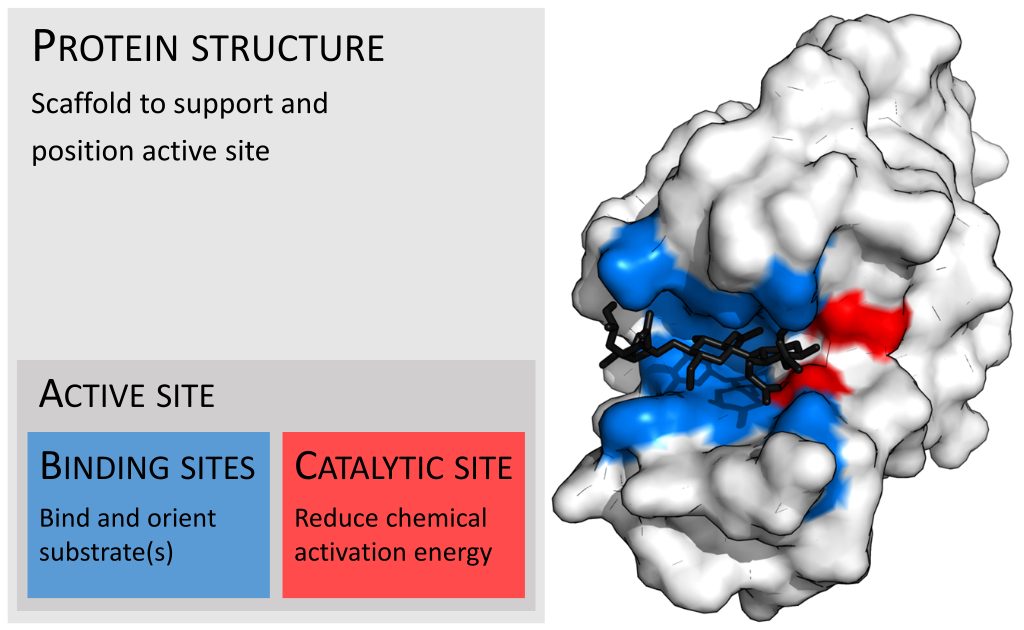
\includegraphics[width=1\textwidth]{img/EnzymeStructure.svg.png}\\
    \source{Thomas Shafee, CC BY 4.0 via Wikimedia Commons}
    \label{fig:EnzymeStructure}
    \end{minipage}
\end{figure}

\begin{itemize}
    \item \textbf{Protein Structure:} The overall structure of the enzyme provides the framework that supports and positions the active site. This structure is critical for the enzyme's stability and functionality. The enzyme's polypeptide chains fold into a unique 3D shape, creating a specific environment for the active site.
    \item \textbf{Active Site:} The active site includes two critical regions: binding sites and the catalytic site. The binding sites (highlighted in blue) are regions where substrates bind to the enzyme. These sites ensure that the substrates are properly oriented for the reaction. The catalytic site (highlighted in red) is the region where the chemical reaction occurs. The catalytic site often contains amino acids with specific functional groups that participate directly in the reaction, reducing the activation energy required for the reaction to proceed.
\end{itemize}

The precise arrangement of amino acids in the active site allows enzymes to be highly specific for their substrates, facilitating efficient catalysis. This specificity is a key feature that enables enzymes to perform their roles in various biochemical pathways with high precision.

A study by Veselovsky et al. (2001) emphasizes the importance of visualizing active site structures, even for enzymes with unknown 3D structures. By analyzing enzyme interactions with reversible competitive inhibitors and molding the substrate-binding region, researchers can predict the shape and dimensions of the active site. This approach has been validated by comparing it with known enzyme-inhibitor complexes, demonstrating its utility in understanding enzyme function and aiding in the search for new ligands.\footcite{veselovskyApproachVisualizationActive2001}

\subsubsection{Role of Enzymes in Biodegradation}
\label{sec:Role of Enzymes in Biodegradation}

Enzymes play a crucial role in the biodegradation of pollutants, including pesticides. The process involves the breakdown of complex organic molecules into simpler, less toxic forms. This degradation is essential for reducing environmental pollution and mitigating the adverse effects of hazardous chemicals.

Hydrolytic Enzymes: Hydrolytic enzymes, such as esterases and amidases, catalyze the cleavage of ester and amide bonds in pesticide molecules. This hydrolysis results in the formation of smaller, more water-soluble compounds that are easier to further degrade and eliminate. For example, microbial esterases can hydrolyze organophosphate insecticides, significantly accelerating their breakdown. \footcite{munneckeEnzymaticHydrolysisOrganophosphate1976a}

Oxidative Enzymes: Oxidative enzymes, such as cytochrome P450 monooxygenases, introduce oxygen atoms into the pesticide molecules, increasing their solubility and reactivity. This oxidation process often converts the pesticides into less harmful substances or intermediates that can be further degraded by other enzymes. The cytochrome P450 enzymes are particularly versatile, capable of metabolizing a wide range of xenobiotics, including pesticides. \footcite{belloTheoreticalApproachMechanism2000}

Reductive Enzymes: Reductive enzymes, including reductases, catalyze the reduction of pesticides, often by adding electrons and hydrogen atoms to the molecules. This reduction can break down complex structures and facilitate the conversion of pesticides into simpler, less toxic forms. Reductive dehalogenases, for instance, play a significant role in the degradation of halogenated organic compounds.

The integration of enzymatic biodegradation with deep learning models can enhance the prediction and analysis of these processes. By using deep learning to analyze enzyme-substrate interactions and their corresponding (EC) classification, we can develop more accurate and efficient bioremediation strategies.

\subsection{Fundamentals of Machine Learning and Deep Learning}
\label{sec:Fundamentals of Deep Learning}

Machine Learning and Deep Learning are two powerful techniques in the realm of machine learning, each offering unique strengths for different types of data and prediction tasks. While deep learning excels at handling unstructured data and automatically extracting features, Machine Learning e.g. Random Forest is known for its robustness, interpretability, and effectiveness in handling structured data with high-dimensional features. This section focuses on the use of Random Forest for sequence-based predictions, particularly in the context of predicting enzyme classes based on protein sequences.

\subsubsection{Introduction to Deep Learning}
\label{sec:Introduction to Deep Learning}

Deep learning has dramatically transformed various fields by enabling the analysis and interpretation of complex datasets. Unlike traditional machine learning methods, which often require manual feature extraction, deep learning models can automatically learn relevant features from raw data. This capability is largely due to the hierarchical structure of neural networks, which can capture multiple levels of abstraction.

A deep neural network is composed of an input layer, multiple hidden layers, and an output layer. Each layer consists of nodes (neurons) that are interconnected with nodes from the previous and next layers. The strength of these connections is determined by weights, which are adjusted during the training process to minimize prediction error. The training is typically performed using a variant of stochastic gradient descent (SGD) and backpropagation, a method for computing the gradient of the loss function with respect to each weight. \footcite{bishopPatternRecognitionMachine2006}

The following image illustrates the basic structure of a deep neural network:

\begin{figure}[hbt]
    \centering
    \begin{minipage}[t]{.9\textwidth}
    \caption{Diagram of a multi-layer feedforward artificial neural network.}
    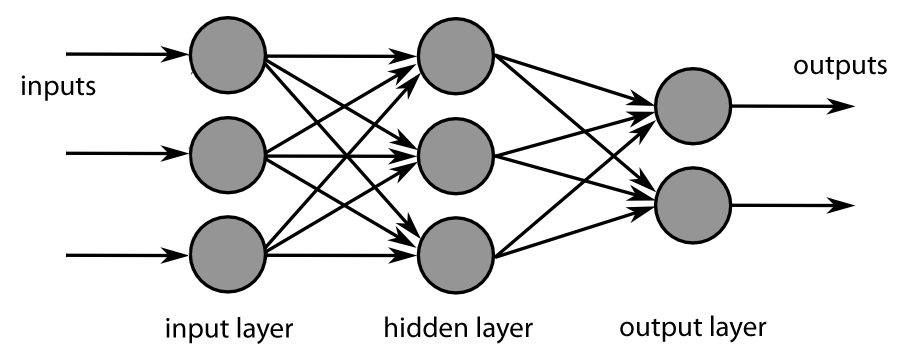
\includegraphics[width=1\textwidth]{img/MultiLayer Neural Network Bigger.png}\\
    \source{Chrislbderivative work, CC BY-SA 3.0 via Wikimedia Commons}
    \label{fig:feedforward_neural_network}
    \end{minipage}
\end{figure}

In this structure, the input layer receives raw data. This data is then processed through one or more hidden layers, where the neurons apply weights and activation functions to capture complex patterns and features. Finally, the processed information reaches the output layer, where the final prediction or classification is made.

Deep learning is particularly effective for problems involving high-dimensional and unstructured data, such as images, audio, and text. Its ability to automatically extract and learn complex features from raw data makes it superior to traditional machine learning methods, which often rely on manually engineered features that may not capture the full complexity of the data.

\subsubsection{Fundamentals of Ligand Binding Site Prediction}
\label{sec:Fundamentals of Ligand Binding Site Prediction}

As mentioned earlier, enzymes interact with substrates at specific binding sites, where the catalytic reactions occur. Predicting these ligand-binding sites is crucial for understanding enzyme function and substrate specificity. Several computational methods have been developed to predict ligand-binding sites from protein structures, including geometric, physicochemical, and machine learning-based approaches.

P2Rank is a machine learning-based tool designed for the rapid and accurate prediction of ligand binding sites from protein structures. It employs a combination of geometric and physicochemical descriptors to analyze protein structures and predict the locations of potential binding sites. P2Rank uses a random forest algorithm, an ensemble learning method that constructs multiple decision trees during training and outputs the mode of the classes (classification) or mean prediction (regression) of the individual trees.

The tool focuses on the interactive parts of enzymes, particularly the ligand-binding sites and the specific amino acids involved. This detailed analysis allows for accurate predictions of enzyme classes and their associated degradation pathways. P2Rank's ability to quickly and accurately predict binding sites makes it a valuable tool for drug discovery and environmental bioremediation applications.

The following image illustrates the workflow of P2Rank, highlighting the process of predicting ligand binding sites from protein structures:

-- P2Rank Workflow --

P2Rank's approach can significantly enhance the accuracy of predicting enzyme-mediated degradation of pesticides by providing detailed insights into the binding interactions at the molecular level. This integration of deep learning and enzyme analysis forms a robust framework for developing bioremediation strategies and understanding the environmental fate of various pollutants. \footcite{krivakP2RankMachineLearning2018}

\subsubsection{Sequence-Based Machine Learning}
\label{sec:Sequence-Based Machine Learning}

In this thesis context, sequence-based machine learning refers to the use of protein sequences as input data for predicting enzyme classes. The sequences are typically represented as strings of amino acids, with each amino acid corresponding to a specific position in the sequence. Machine learning models, such as Random Forest, can analyze these sequences and extract relevant features to predict the enzyme class. This approach uses a Random Forest algorithm, an ensemble learning method that operates by constructing a multitude of decision trees during training and outputting the mode of the classes (classification) or mean prediction (regression) of the individual trees. This method was introduced by Leo Breiman in 2001 and has since become a staple in bioinformatics and other scientific fields due to its versatility and performance. \footcite{breimanRandomForests2001}

The workflow for sequence-based machine learning involves the following steps:

\begin{enumerate}
    \item \textbf{Feature Extraction}: The sequence data, such as amino acid sequences, are first transformed into numerical features. This can include k-mer counts, physicochemical properties of amino acids, and other sequence-derived features.
    \item \textbf{Model Training}: These features are used to train the Random Forest model, which learns to associate specific patterns in the sequence data with enzyme classes.
    \item \textbf{Prediction}: Once trained, the model can predict the enzyme class of new, unseen sequences.
\end{enumerate}

A significant advantage of using Random Forest in this context is its ability to handle complex interaction structures and high-dimensional feature spaces, which are common in biological sequence data. \footcite{diaz-uriarteGeneSelectionClassification2006}

In the context of this study, deep learning techniques are utilized for predicting ligand-binding sites, which are crucial for understanding protein function and interaction with other molecules. Tools like p2rank can be used to predict these binding sites from protein structures, providing the base for a Random Forest model to predict the enzyme class based on the identified ligand-binding sites. This combined approach leverages the strengths of deep learning for feature extraction and Random Forest for classification, enhancing the accuracy and reliability of enzyme class predictions

\subsubsection{Evaluation of Machine Learning Models}
\label{sec:Evaluation of Machine Learning Models}

Evaluating deep learning models involves several metrics and techniques to ensure their accuracy and generalizability. This is essential not only for validating the model’s performance but also for comparing it against other models. Using independent datasets for benchmarking is crucial to demonstrate the model's robustness and applicability to real-world scenarios. Several key metrics are commonly used to evaluate deep learning models:

\begin{enumerate}
    \item \textbf{Accuracy:} The ratio of correctly predicted instances to the total instances. It provides a straightforward measure of performance but can be misleading if the data is imbalanced. \footcite{AccuracyPrecision2024}
    \item \textbf{Precision:} The ratio of true positive predictions to the total predicted positives. Precision is crucial when the cost of false positives is high.
    \item \textbf{Recall (Sensitivity):} The ratio of true positive predictions to the total actual positives. Recall is important when the cost of false negatives is high. \footcite{PrecisionRecall2024}
    \item \textbf{F1-Score:} The harmonic mean of precision and recall, providing a single metric that balances both. It is useful when there is an uneven class distribution. \footcite{Fscore2024}
    \item \textbf{ROC-AUC (Receiver Operating Characteristic - Area Under Curve):} A performance measurement for classification problems at various threshold settings. It tells how much the model is capable of distinguishing between classes. \footcite{ReceiverOperatingCharacteristic2024}
\end{enumerate}

Using these metrics, the performance of deep learning models can be tested on independent datasets. This is critical for ensuring that the models are not just overfitting to the training data but can generalize well to new, unseen data.

In the context of comparing different models, these metrics allow for a standardized evaluation process. By applying the models to benchmark datasets, researches can objectively measure and compare their performance. For instance, in the case of predicting enzyme-mediated pesticide degradation, using independent datasets ensures that the model’s predictions are reliable and can be generalized across various enzyme and pesticide types.

Model evaluation is essential for several reasons: \footcite{emmert-streibIntroductoryReviewDeep2020}

\begin{enumerate}
    \item \textbf{Validation of Model Performance:} Ensuring that the model performs well not just on the training data but also on new, unseen data. This is crucial for the model's reliability and applicability in real-world scenarios.
    \item \textbf{Comparison with Other Models:} By using standardized evaluation metrics and independent datasets, we can objectively compare the performance of different models. This helps in identifying the most effective model for a given task.
    \item \textbf{Identification of Overfitting:} Evaluating the model on independent datasets helps in identifying overfitting, where the model performs well on training data but poorly on new data. Regularization techniques and cross-validation can be used to mitigate this issue.
    \item \textbf{Continuous Improvement:} Regular evaluation allows for continuous monitoring and improvement of the model. Feedback from evaluation metrics can guide further tuning and optimization of the model.
    \item \textbf{Transparency and Trust:} Providing clear and objective evaluation metrics builds trust with stakeholders and users of the model. It ensures that the model’s predictions are transparent and can be trusted for decision-making.
\end{enumerate}

Using benchmark datasets and standardized metrics is a best practice in machine learning and deep learning. It ensures that the models are robust, reliable, and ready for deployment in practical applications. In the context of environmental science and bioremediation, such rigorous evaluation is crucial for developing effective and reliable models for predicting pesticide degradation and other complex processes.
\section{Methodology}
% \addcontentsline{toc}{section}{Methodology}
\fancyhead[R]{Methodology}

\subsection{Data Collection}
\label{sec:Data Collection}

Data collection is a critical step in developing predictive models, as the quality and relevance of the data directly impact the model's performance. In this thesis, the data was collected from Uniprot, a comprehensive resource for protein sequence and functional information. The focus was on obtaining high-quality, reviewed entries with 3D structural data and catalytic properties to ensure the reliability and applicability of the data for predicting enzyme functions. \autocite{uniprotconsortiumUniProtUniversalProtein2021}

Uniprot, or the Universal Protein Resource, is a central repository of protein sequence and annotation data. It is widely recognized for its comprehensive, high-quality data, making it an essential resource for bioinformatics and computational biology. Uniprot integrates information from various sources, including experimental studies, computational analysis, and literature, providing a rich and reliable dataset for scientific research.
Key features of Uniprot include:

\begin{enumerate}
    \item Comprehensive Protein Data: Uniprot contains a vast collection of protein sequences, functional annotations, and cross-references to other databases, making it a valuable resource for protein research.
    \item Reviewed Entries: Uniprot contains both reviewed (Swiss-Prot) and unreviewed (TrEMBL) entries. Reviewed entries are manually curated by experts, ensuring high accuracy and reliability.
    \item Functional Annotations: Each protein entry includes detailed functional annotations, such as catalytic activity, biological processes, and involvement in pathways.
    \item 3D Structural Data: Uniprot links to structural databases like PDB (Protein Data Bank), providing access to 3D structures of proteins, which are crucial for understanding enzyme mechanisms.
    \item Cross-references: Extensive cross-references to other databases (e.g., PDB, BRENDA, Reactome) enhance the richness of the data.
\end{enumerate}

For this study, Uniprot was chosen due to its high-quality data, extensive coverage of protein information, and user-friendly interface. The data collection process involved querying Uniprot for enzyme entries with 3D structural data and catalytic activity annotations, extracting relevant information, and preprocessing the data for model development. The next sections describe the data preprocessing, feature engineering, and model development steps in detail.

The data retrieval process involved using the Uniprot REST API to download protein data that matched specific criteria. The criteria included reviewed entries with both 3D structural data and catalytic properties. The Python script below was used to automate the data retrieval and preprocessing steps:  \autocite{polleyTobiasPolDeepZyme2024}

\begin{figure}[bht]
\begin{lstlisting}[caption=Python script for data retrieval and preprocessing from Uniprot, label=lst:uniprot_data_retrieval]

import requests
from tqdm import tqdm
import gzip
from io import BytesIO
import pandas as pd

base_url = "https://rest.uniprot.org/uniprotkb/search?compressed=true&
fields=accession%2Creviewed%2Cid%2Cprotein_name%2Cgene_names%2Corganism_name%
2Cec%2Corganism_id%2Crhea%2Cxref_alphafolddb%2Cxref_pdb%2Cxref_brenda%
2Cxref_biocyc%2Cxref_pathwaycommons%2Cxref_sabio-rk%2Cxref_reactome%
2Cxref_plantreactome%2Cxref_signor%2Cxref_signalink%2Cxref_unipathway&
format=tsv&query=%28*%29+AND+%28reviewed%3Atrue%29+AND+%28proteins_with%
3A1%29+AND+%28proteins_with%3A13%29"

size = 500
offset = 0
all_data = []

response = requests.get(f"{base_url}&size=1")
if response.status_code == 200:
    total_results = int(response.headers.get("x-total-results", 0))
else:
    print(f"Fehler beim Abrufen der Daten: {response.status_code}")
    total_results = 0

with tqdm(total=total_results, desc="Abrufen der Daten", unit=" Eintrag") as pbar:
    while offset < total_results:
        url = f"{base_url}&size={size}&offset={offset}"
        response = requests.get(url)
        
        if response.status_code == 200:
            with gzip.GzipFile(fileobj=BytesIO(response.content)) as f:
                data = f.read().decode('utf-8')
            if not data.strip():
                break
            all_data.append(data)
            offset += size
            pbar.update(size)
        else:
            print(f"Fehler beim Abrufen der Daten: {response.status_code}")
            break

combined_data = "\n".join(all_data)

df = pd.read_csv(BytesIO(combined_data.encode('utf-8')), sep='\t')

\end{lstlisting}
\end{figure}


\begin{compactenum}
    \item API Request: The script constructs a query to the Uniprot REST API to retrieve reviewed protein entries with specified fields and criteria.
    \item Data Retrieval: Data is retrieved in compressed format and decompressed using gzip.
    \item Data Parsing: The decompressed data is read into a Pandas DataFrame.
    \item Data Filtering: The DataFrame is filtered to retain entries with non-null EC numbers and PDB codes.
    \item Data Splitting: Entries with multiple PDB codes are split into separate rows for each PDB code.
    \item Data Saving: The processed data is saved as a TSV file for further analysis.
\end{compactenum}

\subsection{Data Preprocessing}
\label{sec:Data Preprocessing}

Data preprocessing is a crucial step in preparing the dataset for the prediction model. It involves the protein structure download, p2rank workflow, sequence extraction and combination the data into a single dataset.
The first step in data preprocessing is to download the 3D protein structures from the Protein Data Bank (PDB) using the PDB ID obtained from Uniprot. The PDB is a repository of experimentally determined protein structures, providing valuable insights into the 3D organization of proteins. The structures are needed for the p2rank workflow, which predicts the interactive site residues in the protein structures.

\begin{figure}[bht]
\begin{lstlisting}[caption=Python script for downloading the pdb structure, label=lst:rcsb-data-retrieval]
    def download_pdb(pdb_id):
        pdb_url = f"https://files.rcsb.org/download/{pdb_id}.pdb"
        retries = 3
        for attempt in range(retries):
            try:
                response = requests.get(pdb_url, timeout=10)
                if response.status_code == 200:
                    with open(f'../data/data_preparation/raw_pdbs/{pdb_id}.pdb', 'w') as file:
                        file.write(response.text)
                    return f"Download of {pdb_id} successful."
                else:
                    return f"Fehler beim Herunterladen der PDB-Datei {pdb_id}: {response.status_code}"
            except requests.exceptions.RequestException as e:
                if attempt < retries - 1:
                    continue
                else:
                    return f"Error while downloading {pdb_id}: {e}"

    with ThreadPoolExecutor(max_workers=10) as executor:
        results = list(tqdm(executor.map(download_pdb, pdb_ids), total=len(pdb_ids), desc="Herunterladen der PDB-Dateien"))
\end{lstlisting}
\end{figure}

This script performs the following steps:
\begin{enumerate}
    \item requests.get: Sends an HTTP GET request to the PDB URL to download the protein structure file.
    \item Retry Logic: Attempts to download the file up to three times in case of failures.
    \item File Writing: Saves the downloaded PDB file to the specified directory if the download is successful.
\end{enumerate}

The ThreadPoolExecutor is used to parallelize the download process and speed up the data retrieval.

The next step in data preprocessing is to run the p2rank workflow on the downloaded protein structures to predict the interactive site residues. With the following lines of code, the p2rank workflow is executed on the directory containing the PDB files:

\begin{figure}[bht]
\begin{lstlisting}[caption=Command Line for running p2rank on a given directory, label=lst:p2rank-workflow]
    !./prank.sh predict /Users/tobias.polley/Repositories/DeepZyme/data/data_preparation/raw_pdbs/dataset.ds -o /Users/tobias.polley/Repositories/DeepZyme/data/predictions
\end{lstlisting}
\end{figure}

\subsection{Feature Engineering}
\label{sec:Feature Engineering}

Feature engineering is a critical step in preparing data for prediction models. This process involves transforming raw data into meaningful features that can improve the performance of the model. In this section, the author describes the feature engineering techniques used in this study, focusing on the processing of protein sequences and the calculation of additional features to enhance the predictive power of the Deep Learning model.

To capture meaningful information from protein sequences, this study used several features derived from the sequences, including amino acid composition, molecular weight, isoelectric point, hydrophobicity, and sequence length. These features provide valuable insights into the physicochemical properties of the proteins, enabling the model to learn patterns that correlate with enzyme functions. The ProteinAnalysis class ferom the Biopython library was used to calculate these features. The following Python code snippet demonstrates the calculation of additional features from the protein sequences:

\begin{figure}[bht]
    \begin{lstlisting}[language=Python]
            def calculate_features(sequence):
                sequence = clean_sequence(sequence)
                analysis = ProteinAnalysis(sequence)
                amino_acid_composition = list(analysis.get_amino_acids_percent().values())
                molecular_weight = analysis.molecular_weight()
                isolectric_point = analysis.isoelectric_point()
                hydrophobicity = analysis.gravy()
                sequence_length = len(sequence)
                return amino_acid_composition + [molecular_weight, isolectric_point, hydrophobicity, sequence_length]
    
            additional_features = df["sequence"].apply(calculate_features)
            additional_features = np.array(additional_features.tolist())
\end{lstlisting}
\caption{Source: \autocite{polleyTobiasPolDeepZyme2024}}
\end{figure}

The first step is to clean the protein sequence shown in chapter \ref{sec:Data Preprocessing}. The sequence itself is used as a feature, and additional features are calculated using the ProteinAnalysis class from Biopython. To convert the cleaned sequences into a format suitable for the model, a tokenizer is used to encode the sequences into numerical data. In the context of protein sequences, each amino acid is mapped to a unique integer. For example, the sequence "ACDEFGHIKLMNPQRSTVWY" is tokenized into a list of integers. 

Tokenization involves converting each amino acid into an integer based on its position in a predefined list of valid amino acids. This process can be mathematically represented as:
token $(x) = i $ where $ x \epsilon \{  A , C , D , E , F , G , H , I , K , L , M , N , P , Q , R , S , T , V , W , Y \}$ where $i$ is the index of the amino acid $x$ in the list.

The tokenized sequence is then passed through an embedding layer that transforms these integers into dense vectors. This embedding process is essential for capturing the contextual meaning of each amino acid within the sequence:
$embedding(i) = v$ where $v_i$ is the embedding vector for the token $i$.
These embeddings are fed into the RNN, which processes the sequence and updates its hidden states accordingly, allowing the model to capture complex dependencies and interactions between amino acids. The sequences are then padded to ensure they all have the same length, which is necessary for batch processing in Deep Learning models.

\begin{figure}[bht]
    \begin{lstlisting}[language=Python]
        tokenizer = Tokenizer()
        tokenizer.fit_on_texts(sequences)
        encoded_sequences = tokenizer.texts_to_sequences(sequences)
        
        max_sequence_length = max([len(seq) for seq in encoded_sequences])
        padded_sequences = pad_sequences(encoded_sequences, maxlen=max_sequence_length, padding="post")
\end{lstlisting}
\caption{Source: \autocite{polleyTobiasPolDeepZyme2024}}
\end{figure}

Recent advancements have demonstrated that sequence-based models, including language models like ESM-1b, can achieve high accuracy in predicting protein functions and properties. For instance, the study by Hu et al. (2022) highlights the potential of protein-sequence based models like ESM-1b in predicting protein function from sequences. \autocite{huExploringEvolutionbasedFree2022}

In addition to tokenizing the protein sequences, several biochemical features are calculated to provide a comprehensive representation of the proteins. These features include amino acid composition, molecular weight, isoelectric point, hydrophobicity, and sequence length. The Python code for calculating these features is as follows:

\begin{enumerate}
    \item \textbf{Amino Acid Composition}: The amino acid composition represents the relative frequency of each of the 20 standard amino acids in a protein sequence.
    \begin{enumerate}
        \item Calculation: It is calculated as the percentage of each amino acid in the sequence.
        \item Relevance: Different proteins have characteristic amino acid compositions that can provide clues about their function and stability. For example, membrane proteins often have higher hydrophobic amino acid content.
        \item Example: A protein with a high proportion of hydrophobic amino acids might be involved in membrane-related processes.
    \end{enumerate}
    \item \textbf{Molecular Weight}: Molecular weight is the total mass of all amino acids in the protein sequence.
    \begin{enumerate}
        \item Calculation: It is calculated by summing the average atomic masses of the amino acids in the sequence.
        \item Relevance: The molecular weight of a protein can influence its physical and chemical properties, such as solubility and interaction with other molecules.
        \item Example: Enzymes with larger molecular weights may have multiple domains or subunits.
    \end{enumerate}
    \item \textbf{Isoelectric Point}: The isoelectric point is the pH at which the protein carries no net electrical charge.
    \begin{enumerate}
        \item Calculation: It is determined by calculating the pH at which the positive and negative charges on the amino acids balance out.
        \item Relevance: The pI affects protein solubility and interaction with other molecules. Proteins are least soluble at their pI and more likely to precipitate.
        \item Example: Proteins with a low pI are often found in acidic environments, such as lysosomal enzymes.
    \end{enumerate}
    \item \textbf{Hydrophobicity (GRAVY Score)}: The GRAVY (Grand Average of Hydropathicity) score is a measure of the overall hydrophobic or hydrophilic nature of a protein.
    \begin{enumerate}
        \item Calculation: It is calculated by averaging the hydropathy values of all amino acids in the sequence.
        \item Relevance: Hydrophobicity influences protein folding, stability, and interaction with membranes.
        \item Example: Transmembrane proteins typically have a high GRAVY score due to their hydrophobic transmembrane regions.
    \end{enumerate}
    \item \textbf{Sequence length}: The sequence length is the total number of amino acids in the protein sequence.
    \begin{enumerate}
        \item Calculation: It is simply the count of amino acids in the sequence.
        \item Relevance: The length of a protein can indicate its complexity and the number of functional domains.
        \item Example: Longer proteins may have multiple functional domains or be involved in complex regulatory mechanisms.
    \end{enumerate}
\end{enumerate}

These biochemical features provide a multi-dimensional representation of protein sequences, capturing both sequence-specific information and physicochemical properties. This feature-set is essential for analyzing the enzymes and predicting their functions accurately. A study by Gainza et al. (2020) demonstrates the importance of incorporating physicochemical features in protein function prediction models, showing that these features enhance the model's performance. \autocite{gainzaDecipheringInteractionFingerprints2020}
\subsection{Model Development}
\label{sec:Model Development}


\subsubsection{Model Evaluation}
\label{sec:Model Evaluation}
\section{Results}
% \addcontentsline{toc}{section}{Results}
\fancyhead[R]{Results}

\subsection{Model Performance}
\label{sec:Model Performance}

This chapter presents the performance metrics of the developed model before and after the hyperparameter tuning. The model was evaluated at different EC levels to assess its accuracy, recall, and F1 score. These metrics provide insight into the model's initial performance and highlight areas for potential improvement through hyperparameter tuning.

\begin{table}[hbt]
    \centering
    \begin{tabular}{@{}llll@{}}
    \toprule
    \textbf{EC Level} & \textbf{Accuracy} & \textbf{Recall} & \textbf{F1} \\ \midrule
    1                 & 0.94              & 0,94            & 0,93        \\
    2                 & 0,90              & 0,90            & 0,90        \\
    3                 & 0,94              & 0,94            & 0,93        \\
    4                 & 0,75              & 0,75            & 0,72        \\ \bottomrule
    \end{tabular}
    \caption{Model Performance before Hyperparametertuning}
    \label{tab:performance-before-tuning}
\end{table}

Initial results suggest that the model performs well at higher levels of the EC hierarchy (levels 1 to 3), but there is a notable decrease in performance at the most specific level (level 4). This suggests that there is room for improvement, particularly in fine-tuning the model for more specific classifications. Predicting the 4th EC Level is significantly more challenging than predicting higher levels due to the need to select from approximately 7000 classes \ref{tab:ec-level-distribution}, increasing the difficulty of accurate prediction. Moreover, the model has to predict the right class from a very unbalanced dataset, which makes it even more challenging.

To adress this issue, the model was fine-tuned using a grid search approach to optimize the hyperparameters. In addition to that the initial dataset was edited with the help of the SMOTE algorithm to balance the dataset. The results of the hyperparameter tuning are shown in the following table. \autocite{chawlaSMOTESyntheticMinority2002}
The following table shows the performance of the model after the hyperparameter tuning:

--- NEEDS TO BE DONE ---

\subsection{Comparative Analysis with Existing Models}
\label{sec:Comparative Analysis with Existing Models}

--- NEEDS TO BE DONE ---

\subsection{Interpretation of Model Predictions}
\label{sec:Interpretation of Model Predictions}

--- NEEDS TO BE DONE ---
\section{Discussion}
% \addcontentsline{toc}{section}{Discussion}
\fancyhead[R]{Discussion}

\subsection{Implications of Findings}
\label{sec:Implications of Findings}

The findings of this study have substantial implications for both the field of computational biology and the practical application of Deep Learning models in environmental science. By developing a Deep Learning model that accurately predicts enzyme classes responsible for pesticide degradation, this research contributes to several critical areas.

Traditional methods of determining pesticide degradation and enzyme classification are often labor-intensive, time-consuming, and expensive. The computational approach presented in this study offers a more efficient alternative. By leveraging Deep Learning models, the research significantly reduces the time and cost associated with experimental methods. This efficiency can accelerate the development and testing of new agricultural products, ensuring that safer and more effective solutions reach the market faster.

The model developed in this study demonstrates significant improvements in predictive accuracy, particularly for the 4th level of the Enzyme Commission EC classification hierarchy. This enhanced accuracy is crucial for advancing the understanding of enzyme functions and their specific roles in biodegradation processes. Accurately predicting enzyme classes allows for more precise identification of enzymatic pathways involved in pesticide degradation, which is fundamental for developing effective bioremediation strategies. The Deep Learning model can be employed to help predicting unknown enzyme classifications in order to clean up contaminated environments more efficiently and reduce the ecological footprint of agricultural practices. The findings support the creation of more sustainable and environmentally friendly agricultural products, aligning with global efforts to mitigate pollution and protect natural ecosystems. At Bayer Crop Science, the model can be integrated into the product development process to enhance the safety and sustainability of new agricultural products, reducing the environmental impact of pesticide use. Especially in the modern context of increasing environmental awareness and regulatory scrutiny, the model provides a valuable tool for the development of new enzymes and biodegradation pathways.

The findings open several avenues for future research. One potential direction is the refinement of the model to improve performance at the fourth EC level, which remains challenging due to the high specificity and diversity of enzyme functions. Additionally, integrating this model with real-world environmental data can validate its practical applicability and uncover further insights into enzymatic degradation pathways. Collaborative efforts with experimental biologists can enhance the model's accuracy and expand its scope to include a wider range of pollutants and environmental conditions.

Moreover, this novel approach can be further improved to achieve even better results. Current methods often utilize the entire protein sequence and do not focus specifically on the ligand-binding pocket. By concentrating more on these specific pockets, it is possible to enhance the precision of enzyme classification and the prediction of degradation pathways. Future advancements should therefore aim to refine this focus on ligand-binding sites, leveraging detailed structural information to improve predictive accuracy.


\subsection{Strenths and Limitations}
\label{sec:Strenths and Limitations}

\textbf{Strengths:}

\begin{enumerate}
    \item Innovative Approach: The primary strength of this thesis lies in its innovative approach to predicting pesticide degradation by focusing on enzyme classification through Deep Learning. By integrating advanced computational techniques, this research addresses a gap in the current methodologies used for enzyme function prediction.
    \item Comprehensive Methodology: The detailed and methodical approach taken in data collection, preprocessing, feature engineering, and model development ensures the robustness of the study. Each step is meticulously documented, demonstrating a thorough understanding of the processes involved in developing a predictive model.
    \item Utilization of Advanced Tools: The use of state-of-the-art tools such as P2Rank for ligand-binding site prediction and RNNs for sequence analysis highlights the technical sophistication of the study. These tools provide a solid foundation for accurate predictions and demonstrate the potential for further applications in bioinformatics.
    \item Significant Performance Improvement: The developed model shows significant improvement in predictive accuracy, particularly at the higher levels of the Enzyme Commission hierarchy. This improvement underscores the effectiveness of combining sequence-based features with additional biochemical features.
    \item Environmental and Economic Impact: By enabling more accurate predictions of pesticide degradation pathways, the study contributes to environmental sustainability and cost efficiency. The ability to develop targeted bioremediation techniques and accelerate the development of environmentally friendly agricultural products has far-reaching benefits.
\end{enumerate}

\textbf{Limitations:}

\begin{enumerate}
    \item Performance at Specific EC Levels: While the model performs well at higher EC levels, there is a notable decrease in performance at the most specific level (level 4). This limitation suggests that the model struggles with the high specificity and diversity of enzyme functions at this level, necessitating further refinement and optimization. One of the reasons is that the UniProt database is still unbalanced and needs to be further improved. In addition to that, it is possible that some enzymes are wrongly classified in the database, which can lead to wrong predictions.
    \item Imbalanced Dataset: The initial dataset used in the study is highly imbalanced, with certain enzyme classes being significantly underrepresented. Although techniques such as SMOTE were employed to address this issue, the imbalance may still affect the model's ability to generalize across all enzyme classes.
    \item Focus on Ligand-Binding Pockets: Although the study emphasizes the importance of ligand-binding pockets, current methods still utilize the entire protein sequence, which may dilute the specificity of predictions. Future research should aim to enhance the focus on these pockets to improve predictive accuracy.
    \item Generalizability to Real-World Data: The model's performance is primarily evaluated using data from UniProt and PDB, which are well-curated databases. The generalizability of the model to real-world environmental data remains to be validated, as real-world scenarios often involve more complex and noisy data. Although the model needs to be validated in vivo or in vitro, the results are promising and provide a strong foundation for further research.
\end{enumerate}
\section{Conclusion}
% \addcontentsline{toc}{section}{Conclusion}
\fancyhead[R]{Conclusion}

\subsection{Summary of Findings}
\label{sec:Summary of Findings}

In this thesis, a novel Deep Learning model was developed to predict the enzymatic function based on the protein sequence. The research addressed the need for more accurate and efficient methods to predict enzyme classes responsible for pesticide degradation. The key findings of the research are summarized as follows:

\begin{enumerate}
    \item Novel Deep Learning Model: The developed Deep Learning model leverages enzyme binding site predictions to enhance the accuracy of enzyme class predictions. This approach focuses specifically on the ligand-binding sites, offering a more detailed and precise prediction by targeting critical interaction regions. With the use of the p2rank tool, the model can identify specific residues involved in catalytic processes, improving the accuracy of enzyme class predictions. Focussing on ligand-binding pockets has shown to be more effective than traditional methods that utilize the entire protein sequence.
    \item Data Preprocessing and Feature Engineering: Comprehensive data preprocessing steps, including cleaning, tokenization, and padding of sequences, ensured the dataset's quality and consistency. Feature engineering incorporated biochemical properties such as molecular weight, isoelectric point, hydrophobicity, and sequence length, which significantly contributed to the model's predictive power. The inclusion of these features enhance the model's ability to learn from the data and make accurate predictions.
    \item Handling Data Imbalance: The study addressed the dataset's imbalance using the RandomUnderSampler algorithm, which improved the model's ability to learn from underrepresented classes, although further optimization is necessary for perfect balance. There is a need for more data in UniProt to improve the model's performance, particularly for the 4th EC level, which has a large number of classes and is challenging to predict accurately. As shown in chapter \ref{sec:Data Preprocessing}
    \item Model Performance: The model demonstrated high predictive accuracy, particularly at the first four levels of the Enzyme Commission (EC) hierarchy. Existing models struggle to predict the 4th EC level due to the large number of classes and the dataset's imbalance. The developed model showed promising results at this level, indicating its potential to accurately predict enzyme classes in detail. The model's performance was further improved through hyperparameter tuning and data balancing techniques.
    \item Implications for Environmental Science: The findings highlight the model's potential to accelerate the development of environmentally friendly agricultural products by reducing the time and cost associated with experimental methods. Accurate enzyme class predictions facilitate better risk assessments and the development of sustainable bioremediation strategies.
\end{enumerate}

This thesis makes significant contributions to the fields of computational biology and environmental science by developing an innovative Deep Learning model. By leveraging modern Deep Learning techniques, this study enhances the accuracy and efficiency of enzyme function predictions, offering a substantial improvement over traditional methods. Moreover the model could save time and money in the development of new products, as well as reduce the risk of harmful pesticides in the environment.

The practical implications of this research are profound, particularly for sustainable agriculture. By enabling more precise predictions of enzyme-mediated pesticide degradation, the model supports the development of safer and more effective bioremediation strategies. This aligns with global efforts to reduce the environmental impact of pesticide use and promote sustainable agricultural practices. Moreover, the efficiency and accuracy of this model can lead to significant cost savings in the development and testing of new agricultural products, facilitating the faster introduction of environmentally friendly solutions to the market.

In addition to its environmental benefits, the research highlights the economic advantages of biotransformation. Utilizing enzymes to facilitate chemical reactions in pesticide degradation can significantly reduce production costs, making agricultural practices more sustainable and cost-effective. By predicting previously unknown enzyme classes involved in pesticide degradation, this model opens up new opportunities for developing innovative bioremediation solutions that are both environmentally friendly and economically viable. Traditional methods for determining enzyme classes are labor-intensive and time-consuming, making the model a valuable tool for accelerating the discovery of new enzymes and their functions.

\subsection{Final Remarks and Future Work}
\label{sec:Final Remarks and Future Work}

This thesis presents a novel Deep Learning model designed to predict enzyme classes based on their protein sequence. By leveraging detailed biochemical features and focusing on ligand-binding sites, the model demonstrates significant improvements on the first three levels and a slight increase on the 4th level in predictive accuracy compared to existing methods. The comprehensive data preprocessing, integration of sequence-based and property-based features, and the use of Deep Learning techniques such as LSTM layers have proven to be highly effective in capturing the complex nature of enzyme functions. The model's performance was further enhanced through hyperparameter tuning and data balancing techniques, demonstrating its potential to accurately predict enzyme classes. The implications of this research are far-reaching, with significant benefits for environmental science. Unknown enyzmes can be predicted accurately and used to develop new products. The model can also save time and money in the development of new products, as well as reduce the risk of harmful pesticides in the environment.

Despite the significant advancements presented in this thesis, there remains substantial potential for further improvement and refinement of the model. One potential enhancement is the integration of anchor sequences, as utilized in ECPred, to improve the decision-making power of the model. Anchor sequences are specific segments within proteins that are highly conserved and play crucial roles in their function. By focusing on these sequences, the model can gain a deeper understanding of the critical regions that determine enzyme activity. This approach can help in identifying key residues involved in substrate binding and catalysis, thereby improving the accuracy of enzyme classification. Anchor sequences provide essential structural and functional information that can enhance the model's ability to predict enzyme classes. They act as reliable markers for specific enzyme functions, allowing the model to make more informed predictions. Integrating anchor sequences into the feature set can help the model focus on the most relevant parts of the protein, improving its decision-making capabilities.

Another promising direction is the use of embeddings from ProtBERT, a pre-trained language model for protein sequences. ProtBERT embeddings capture rich contextual information from amino acid sequences, enabling the model to understand complex patterns and dependencies within the data. By incorporating these embeddings, the model can leverage the extensive knowledge encoded in ProtBERT, potentially enhancing its predictive performance ProtBERT embeddings provide a comprehensive representation of protein sequences, capturing both local and global sequence information. This can help the model generalize better across different enzyme classes and improve its ability to recognize subtle variations in sequence that are critical for enzyme function.

Further refinement of data augmentation techniques can address the issue of class imbalance more effectively. While RandomUnderSampling has been used in this study, exploring other methods such as SMOTE (Synthetic Minority Over-sampling Technique) or advanced generative models to create synthetic data for underrepresented classes can improve the model's performance on these classes. Also incorporating more diverse biochemical and environmental data can enhance the model's predictive accuracy. For example, integrating data on enzyme kinetics, thermodynamic stability, and environmental factors affecting enzyme activity can provide a more holistic view of enzyme function.

In conclusion, the Thesis represents a significant advancement in the field of enzyme classification. By integrating advanced Deep Learning techniques with detailed biochemical features, the model offers a powerful tool for computational biology. Future research should focus on incorporating anchor sequences, utilizing ProtBERT embeddings, refining data augmentation techniques, integrating additional data, and optimizing the model architecture to further enhance its capabilities and broaden its applicability.
%%%%%%%%%%%%%%%%%%%%%%%%%%%%%%%%%%%%%%%%%%%%%%%%%%%%%%%%%%%%%%%%%%%%%%%

%!TEX root = ../Thesis.tex
\section*{Appendix}
\addcontentsline{toc}{section}{Appendix}
\fancyhead[R]{Appendix}

\appendixlist

\appendix{Filler}

\subappendix{Filler}
\begin{compactitem}
\item \textbf{Filler}
\end{compactitem}

%!TEX root = ../Thesis.tex
\section*{List of references}
\addcontentsline{toc}{section}{List of references}
\fancyhead[R]{List of references}

\defbibheading{mono}{\subsection*{Monographien}}
\defbibheading{mag}{\subsection*{Aufsätze in Sammelbänden und Zeitschriften}}
\defbibheading{article}{\subsection*{Zeitungsartikel}}
\defbibheading{web}{\subsection*{Internetquellen}}
\defbibheading{misc}{\subsection*{Other sources}}

\setlength\bibitemsep{1.5\itemsep}
\setlength{\bibhang}{2em}

\renewcommand{\baselinestretch}{1.50}\normalsize

\begingroup
\sloppy

% \printbibliography[heading=mono,keyword=mono]
% \printbibliography[heading=mag,keyword=mag]
% \printbibliography[heading=web,keyword=web]
\printbibliography[heading=article,keyword=article]
\printbibliography[heading=misc,keyword=misc]

\endgroup

%%%%%%%%%%%%%%%%%%%%%%%%%%%%%%%%%%%%%%%%%%%%%%%%%%%%%%%%%%%%%%%%%%%%%%%

%!TEX root = ../Thesis.tex

\section*{Statement of independent work}
\addcontentsline{toc}{section}{Statement of independent work}
\fancyhead[R]{Statement of independent work}

Hiermit erkläre ich, dass ich die vorliegende \dokumententyp{} selbständig angefertigt habe. Es wurden nur die in der Arbeit ausdrücklich benannten Quellen und Hilfsmittel benutzt. Wörtlich oder sinngemäß übernommenes Gedankengut habe ich als solches kenntlich gemacht. Diese Arbeit hat in gleicher oder ähnlicher Form noch keiner Prüfungsbehörde vorgelegen.
\vspace{20mm}

\ort, \abgabedatum
\vspace{10mm}

\underline{\hspace{8cm}}\\\dokumentenautor

%%%%%%%%%%%%%%%%%%%%%%%%%%%%%%%%%%%%%%%%%%%%%%%%%%%%%%%%%%%%%%%%%%%%%%%

\end{document}
